% Diese Zeile bitte -nicht- aendern.
\documentclass[course=erap]{aspdoc}

%%%%%%%%%%%%%%%%%%%%%%%%%%%%%%%%%
%% TODO: Ersetzen Sie in den folgenden Zeilen die entsprechenden -Texte-
%% mit den richtigen Werten.
\newcommand{\theGroup}{242} % Beispiel: 42
\newcommand{\theNumber}{A505} % Beispiel: A123
\author{Maha Marhag \and Magdalena Papagianni \and Alihan Sencan}
\date{Sommersemester 2022} % Beispiel: Wintersemester 2019/20
%%%%%%%%%%%%%%%%%%%%%%%%%%%%%%%%%

% Diese Zeile bitte -nicht- aendern.
\title{Gruppe \theGroup{} -- Abgabe zu Aufgabe \theNumber}

\begin{document}
\maketitle

\section{Einleitung}


Kryptographie, stammend aus dem altgriechischen \textit{Geheim} und \textit{schreiben}, ist die Wissenschaft der Verschlüsselung von Informationen. Es gibt viele Algorithmen, welche verschlüsselte Kommunikation ermöglichen, aber in dieser Ausarbeitung widmen wir uns dem Message-Digest 2 (MD2) Algorithmus und dessen Eigenschaften, Sicherheitsmerkmale, Angriffsmöglichkeiten und mögliche Alternativen. Im nächsten Kapitel werden wir unsere eigene C Implementierung genauer erläutern und in den weiteren Kapiteln dann auch auf die Korrektheit und die Performanz eingehen.

\subsection{Überblick über den Message-Digest 2 Algorithmus}

Der MD2 ist eine kryptografische Hashfunktion, die 1989 von Ronald Rivest entwickelt wurde \cite{rfc1319}. Eine Hashfunktion ist eine Funktion, die verwendet werden kann, um Nachrichten, Dateien oder Daten (im weiteren Text wird einfachheitshalber nur von Nachrichten gesprochen) beliebiger Größe auf Werte fester Größe abzubilden \cite{hash}.  

Der MD2 Algorithmus wird zum Prüfen von Nachrichten genutzt. Vor allem ist der MD2 Algorithmus für digitalen Signaturen konzipiert worden, in der eine Nachricht auf eine sichere Weise "`komprimiert"' werden kann, bevor sie mit einem privaten Schlüssel signiert wird \cite{rfc1319}. Der Algorithmus akzeptiert eine Nachricht beliebiger Länge als Eingabe $x$ und erzeugt als Ausgabe einen 16-Byte Message Digest $H(x)$, indem er eine gewisse Redundanz an die Nachricht anhängt und dann iterativ eine Komprimierungsfunktion von 48 Bytes auf 16 Bytes anwendet.  \cite{md2Checksum}. MD2 ist ein Byte-orientierter Algorithmus und damit eine der ersten Hashfunktionen, er unterscheidet sich aber deutlich von moderneren Algorithmen wie MD4, MD5, SHA und SHA-1\cite{attack}.

\subsection{Sicherheitseingeschaften}

ryptografische Hashfunktionen sollten folgende drei Sicherheitseigenschaften erfüllen: \cite{Spitz2011}

\begin{itemize}
\item \textbf{Urbildresistenz}: Hashfunktionen müssen nur in eine Richtung funktionieren. Bedeutet, dass für eine Hash-Ausgabe $z$ es rechnerisch unmöglich sein muss, eine Eingabenachricht $x$ zu finden, bei der $z = H(x)$ gilt.
\item \textbf{Zweite Urbildresistenz:} Auch schwache Kollisionsresistenz genannt, besagt, dass zwei verschiedene Nachrichten $x_{1} \neq x_{2}$ nicht den gleichen Hash-Wert haben dürfen $H(x_{1}) \neq H(x_{2})$. Dabei zeichnet sie sich dadurch aus, dass $x_{1}$ gegeben ist und versucht wird $x_{2}$ zu finden.
\item \textbf{Kollisionsresistenz}: Wir nennen eine Hashfunktion kollisionssicher, wenn es rechnerisch nicht möglich ist, zwei verschiedene Eingaben $x_{1} \neq x_{2}$ mit $H(x_{1}) = H(x_{2})$ zu finden. Im Vergleich zur zweiten Urbildresistenz kann in diesem Fall $x_{1}$ und $x_{2}$ frei gewählt werden.
\end{itemize}

\subsection{Angriffe auf der MD2}

Es gibt verschiedene Angriffsarten, die bei der MD2 Hashfunktion erfolgreich durchgeführt wurden. In 2004 wurde ein Erstes-Urbild-Angriff durchgeführt \cite{attack}, 2008 wurde dieser Angriff weiter verbessert \cite{preimageattack} und 2009 folgte der erste Angriff auf Kollisionsresistenz \cite{urbild}. Folgend werden die drei möglichen Angriffsarten auf Hashfunktionen näher beschrieben und erläutert:

\begin{itemize}
\item \textbf{Angriff auf Kollisionsresistenz}: Ziel ist es für unterschiedliche Nachrichten $x_{1}\neq x_{2}$ den selben Hashwert zu errechnen $H(x_{1}) = H(x_{2})$. Bei dieser Art von Angriff berechnet der Angreifer via brute-force-Suche den Hashwert $H(x_{i})$ beliebiger Nachrichten $x_{i}$. Die generierten Hashwerte werden in einer geordneten Liste gespeichert. Der Angriff gilt als erfolgreich, sobald beim Speichern in der Liste ein gleicher Hashwert erkannt wird \cite{Spitz2011}. 

\item \textbf{Urbild-Angriff}: Gegeben sei nur ein Hashwert $H(x_{1})$, Ziel ist es eine Nachricht $x_{2}$ zu finden, so dass $H(x_{2}) = H(x_{1})$ gilt. Dies kann durch eine brute-force-Suche durchgeführt werden\cite{attack}.

\item \textbf{Zweites-Urbild-Angriff}: Gegeben sei eine Nachricht $x_{1}$ und dessen Hashwert $H(m_{1})$. Ziel dieses Angriffs ist es eine Nachricht $x_{2} \neq x_{1}$ zu finden, so dass $H(x_{2}) = H(x_{1})$ gilt. Der Erste-Urbild-Angriff ist auch gleichzeitig ein Zweiter-Urbild-Angriff, da es trivial ist sicherzustellen, dass eine erhaltene Nachricht von einer gegebenen Nachricht abweicht \cite{urbild}.
\end{itemize}

\subsection{Alternativen}

Wie gezeigt wurde ist MD2 keine ausreichend sichere Hashfunktion mehr und aus diesem Grund wurde diese 2011 von der IETF als \textit{"'historisch"'}, also obsolet eingestuft \cite{rfc6149}. Deshalb ist es ratsam andere Alternativen zu verwenden, wie zum Beispiel\cite{Pelzl2016}:
\begin{itemize}
    \item MD5 - ist eine weit verbreite Hashfunktion welche mittlerweile auch als unsicher gilt
    \item SHA-1 - eine weitere weit verbreitete Hashfunktion , die ebenfalls nicht mehr als sicher gilt
    \item SHA-3 - eine relativ neue Hashfunktion , die 2015 standardisiert wurde und im Rahmen eines öffentlichen Wettbewerbs entwickelt wurde
\end{itemize}
SHA-3 ist der aktuellste und sicherste Standard und es ist deshalb ratsam wenn möglich immer SHA-3 zu verwenden \cite{Pelzl2016}.

\section{Lösungsansatz}

In unserer Implementierung der MD2-Hashfunktion, beginnen wir unter der Annahme, dass wir eine $x-$Byte-Nachricht als Eingabe haben. Wir wollen zunächst ihren Message-Digest finden. Dabei ist $x$ eine beliebige, nicht negative Zahl, also darf diese $0$ oder beliebig groß sein. Um den Message-Digest der Nachricht zu berechnen, lesen wir zunächst eine Datei Zeile für Zeile in den Speicher ein. Einen Zeiger auf die Eingabe geben wir dann an eine weitere Funktion weiter, die den Hash berechnet. Dabei verwenden wir Padding, Checksum und Kompression, welche in den nächsten Unterkapiteln genauer erklärt werden.  

\subsection{Padding}

Padding beschreibt das \textit{"`Auffüllen"'} einer Nachricht mit Fülldaten. Die eingegebene Nachricht wird vor der Verschlüsselung in Blöcke geteilt, die eine gleiche und feste Länge von 16 Byte haben. Wenn die eingegebene Nachricht nicht ein Vielfaches der festen Blocklänge ist, wird diese mit entsprechend vielen Bytes, auch Pad-Bytes genannt, aufgefüllt\cite{paddingSchwenk}. Somit wird die Größe der Daten in das akzeptierte und feste Format des gegebenen Algorithmus gebracht \cite{paddingA}. In \autoref{fig:blockvert} wird die Verteilung und das Padding visualisiert. Padding wird verwendet, nicht nur um die benötigen Bytes aufzufüllen, sondern auch um die Sicherheit der Algorithmen und Protokolle zu erhöhen\cite{bundes}\cite{kryptografie}.  \\
Im speziellen verwenden wir in unserer Implementierung den \texttt{PKCS\#7} Standard. Beim \texttt{PKCS\#7} Padding kann die Blocklänge zwischen $1$ und $2^{n-1}$ ($n$ ist die Anzahl der Bytestellen) liegen. Wenn die Anzahl von $n$ Bytes als Pad-Bytes addieren werden, wird das Byte “`$n$”' $n$-mal an den Block konkateniert, wie in \autoref{fig:padbytes} zu sehen ist. $n$ kann zwischen $1$ und der Blocklänge liegen\cite{kryptografie}. Um die Bytes aufzufüllen nutzen wir die Funktion \texttt{memset}. Als konkretes Beispiel in \autoref{fig:padbytes} benötigen wir ein Padding von fünf Byte und füllen deshalb den Nachrichtenblock mit fünf mal der $5$ auf. Würden wir nur ein Padding von vier Byte benötigen, würden wir dann analog mit $4$ auffüllen.

\begin{figure}[H]
    \centering
    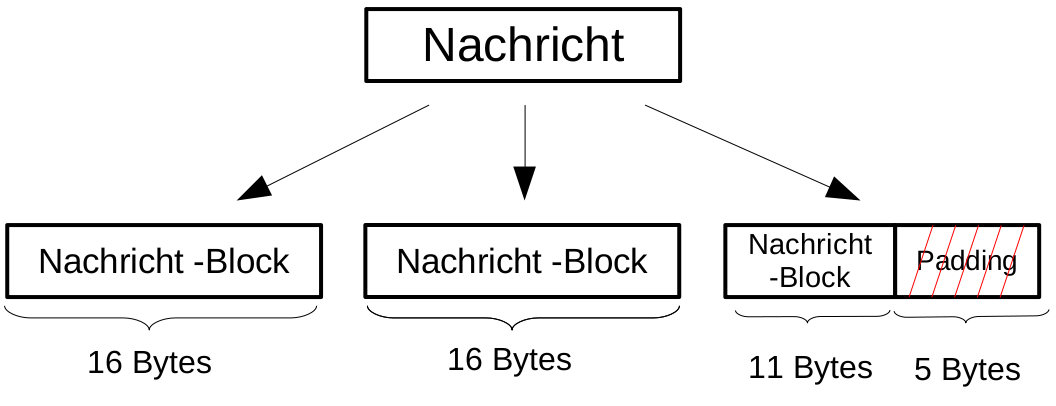
\includegraphics[height=5cm]{Figures/Padding1.png}
    \caption{Block-Verteilung}
    \label{fig:blockvert}
\end{figure}

\begin{figure}[H]
	\centering
	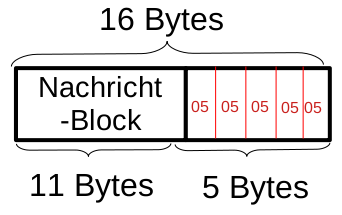
\includegraphics[height=3.5cm]{Figures/Padding2.png}
	\caption{Pad-bytes}
	\label{fig:padbytes}
\end{figure}

\subsection{Checksum}

Eine Prüfsumme (eng.: Checksum) ist definiert als: \textit{"`Eine Zahl, die sich aus der Addition aller Zahlen eines elektronischen Datensatzes ergibt, um die Richtigkeit der Daten zu überprüfen"'}\cite{cambridge}.
Im MD2-Hash-Algorithmus ist die Prüfsumme ein 16-Byte-Block, der an die durch Padding angereicherte Nachricht, angehängt wird. Für das Anhängen der Prüfsumme an das Ende der Nachricht wird eine S-Box verwendet \cite{rfc1319}. Die S-Box ist eine 256-Byte-Zufalls-Permutationstabelle, welche ganze Zahlen von $0$ bis $255$ enthält. Unter Verwendung einer Variante des Durstenfeld-Algorithmus mit einem Pseudozufallszahlengenerator auf der Grundlage der Dezimalziffern von $\pi$ werden diese gemischt und eine zufällige Permutation auf die Folge $a[i]$ mit $i = 1, 2, ..., 256$ angewendet. Der Inhalt der S-Box in hexadezimal wird in \autoref{fig:stabelle} gezeigt \cite{rfc1319}. 

\begin{figure}[H]
    \centering
    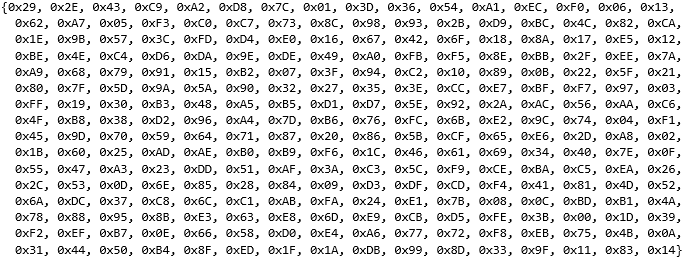
\includegraphics[width=\textwidth]{Figures/S-table.png}
    \caption{S-Box}
    \label{fig:stabelle}
\end{figure}

Zur Berechnung der Prüfsumme, wie in \autoref{fig:checksum} zu sehen ist, verwenden wir ein mit Null initialisiertes 16-Byte-Array (Buffer) und mehrfache \texttt{XOR}-Operationen mit der Prüfsumme (checksum) und der S-Box.

\begin{figure}[H]
    \centering
    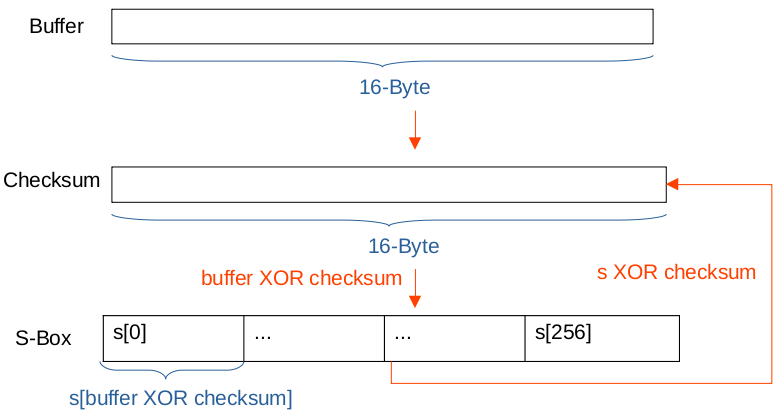
\includegraphics[width=\textwidth]{Figures/checksum.png}
    \caption{Berechnung der Prüfsumme}
    \label{fig:checksum}
\end{figure}


\subsection{Kompressionsfunktion}

Um die Hash-Operationen durchzuführen verwenden wir ein anfangs leeres Output-Array mit einer Größe von 48-Byte, also insgesamt drei mal 16-Byte Blöcke. Der 16-Byte große Input-Buffer wird als Block in den zweiten Block des Output-Arrays kopiert. Anschließend wird mit Hilfe der 256-Byte großen S-Box (siehe \autoref{fig:stabelle}) das Ergebnis mittels \texttt{XOR}-Operationen berechnet. Eine Kompression kommt zustande, weil sich das Ergebnis nur auf der ersten Block des Output Arrays beschränkt. Die Kompressionsfunktion wird auch in \autoref{fig:compress_function} dargestellt. 

\begin{figure}[H]
    \centering
    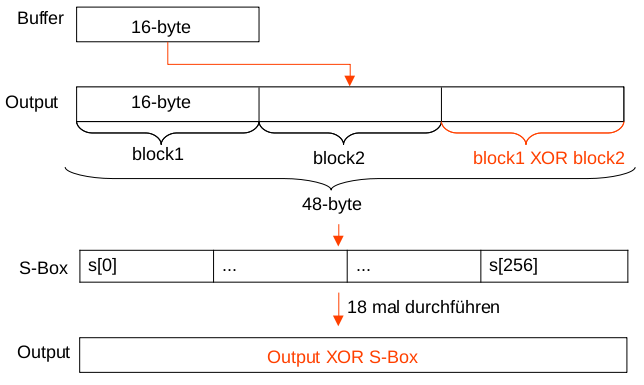
\includegraphics[width=\textwidth]{Figures/compression_function.png}
    \caption{Kompressionsfunktion}
    \label{fig:compress_function}
\end{figure}


\subsection{Lösungsalternative}

Als alternative Implementierung (\texttt{V1}) haben wir eine Lösung mit \texttt{Structs} gewählt. Dies erlaubt Daten unterschiedlicher Typen zu kombinieren, vereinfacht den Aufbau des Quelltexts und erhöht somit die Lesbarkeit und Wartbarkeit des Programms. Diesen Ansatz haben wir nicht als primäre Implementierung gewählt, da wir die vorgegebene Signatur ändern mussten.

\subsection{Optimierungen} \label{ss:opt}

Für die Berechnung eines Hashwertes sind viele Speicherzugriffe erforderlich, da nicht nur die Nachricht beziehungsweise Eingabedatei verarbeitet werden muss, sondern auch fast jeder Zwischenschritt Daten im Speicher verarbeitet. Diese sind die laufzeitintensivsten Operationen in unserer Implementierung und somit der ideale Kandidat, um diese genauer zu Untersuchen und mögliche Optimierungsansätze zu evaluieren und umzusetzen. Folgende konkrete Optimierungen haben wir schließlich implementiert:

\begin{itemize}
    \item Pad-Bytes werden nicht mehr in den Buffer kopiert und iterativ in einer While-Schleife angehangen, sondern mit der Bibliotheksfunktion \texttt{MEMSET} effizient in einem Durchlauf geschrieben 
    \item Die iterative Initialisierung der Arrays mit Null, welche für die Berechnung des Hash verwendet wird, wurde auch durch die \texttt{MEMSET}-Funktion ersetzt
    \item Effizientere vektorisierte \texttt{SIMD-XOR}-Operationen werden eingesetzt, anstatt sequenziell und wiederholt \texttt{XOR}-Operationen aufzurufen
\end{itemize}  

Andere Optimierungen haben wir nicht vorgenommen, da zum Beispiel in \texttt{IO.c} keine Iterationen und Speicherallokationen erfolgen und wir \texttt{Loop-Carried-Dependencies} in den Funktionen \texttt{Checksum} und \texttt{Transform} haben. Weitere Optimierungen wären jedoch möglich gewesen, diese behandeln wir aber näher in \autoref{ss:fazit}.

\section{Korrektheit}

Zur Überprüfung der Korrektheit unserer Ergebnisse haben wir eine Reihe von Tests erstellt. Diese Tests behandelt Eingabedateien verschiedenster Größen und auch einige Randfälle - wie in der untenstehenden Tabelle kurz aufgeführt. Natürlich hat die Größe der Eingabe und der Typ der Zeichen keinen Einfluss auf das Ergebnis, da 16-Byte ausgerichtete Speicherzugriffe (input, output und checksum Arrays) eine 16-Byte Ausgabe garantieren. Neben den Beispielen in der Test Suite des RFCs \cite{rfc1319} haben wir auch mehrere Tests mit Hilfe eines Online MD2-Hashgenerators \cite{onlineHash} erstellt und verifiziert, um eine breiterer Reichweite von Testfällen abzudecken. 

\begin{table}[H]
\resizebox{\textwidth}{!}{
\begin{tabular}[width=\textwidth]{|c|c|}
 \hline
\textbf{Eingabe} & \textbf{Hash}\\
 \hline
       \textit{leere Datei}  &   \texttt{8350e5a3e24c153df2275c9f80692773}         \\ \hline
         \texttt{.... . .-.. .-.. --- / .-- --- .-. .-.. -.. / -.-.-- }  &  \texttt{c6dc54d633087cbe5046d25129e1467c} \\ \hline           
        \texttt{abc }  &  \texttt{da853b0d3f88d99b30283a69e6ded6bb} \\ \hline
         \texttt{ABCDEFGHIJKLMNOPQRSTUVWXYZabcdefghijklmnopqrstuvwxyz0123456789}  &  \texttt{da33def2a42df13975352846c30338cd} \\ \hline
\end{tabular}
}
\end{table}


\section{Performanzanalyse}
\label{perf}
In diesem Kapitel möchte wir die Perfomanzunterschiede unsere Implementierung anhand zweier Umsetzungsversionen erläutern. Dabei handelt es sich um die \textit{optimierte} und die \textit{nicht-optimierte} Version. Die vorgenommenen Optimierungen haben wir bereits in \autoref{ss:opt} näher erläutert. Die Laufzeitvergleiche für die Leistungsanalyse wurden gemäß Abschnitt "`Benchmarking"' des Praktikums durchgeführt. Wie in den Folien angegeben, wurde \texttt{MONOTONIC Clock} verwendet, um die Zeit für die zwei Versionen zu messen. Die optimierte Version hatte nur eine 6-mal schnellere Durchlaufzeit für Eingaben mit weniger als 500 Zeichen. Dies ist dem Umstand geschuldet, dass zusätzliche \texttt{SIMD}-Befehle, die zum Laden und Speichern von Daten verwendet werden, die Laufzeit beeinflussen. Die zusätzlichen Befehle, die für die Speicherregulation nötig sind, verlangsamt die Geschwindigkeit des Programms für kleine Eingaben, da der Overhead in Relation zur Laufzeut mehr ins Gewicht fällt, aber sind sehr vorteilhaft bei größeren Dateneingaben.
Mit wachsender Eingabegröße ist die optimierte Version aber deutlich performanter. Die Zeiten der optimierten Version sind bei Eingaben im fünfstelligen Bereich 20- bis 30-mal schneller als die nicht-optimierte Version und sogar über 70-mal so schnell bei 10.000 Zeichen. In \autoref{fig:perf} sieht man den Vergleich der beiden Implementierungen. Die Zeiten basieren auf mehreren Durchläufen und sind dann anschließen arithmetisch gemittelt worden. 

\begin{figure} [H]
    \centering
    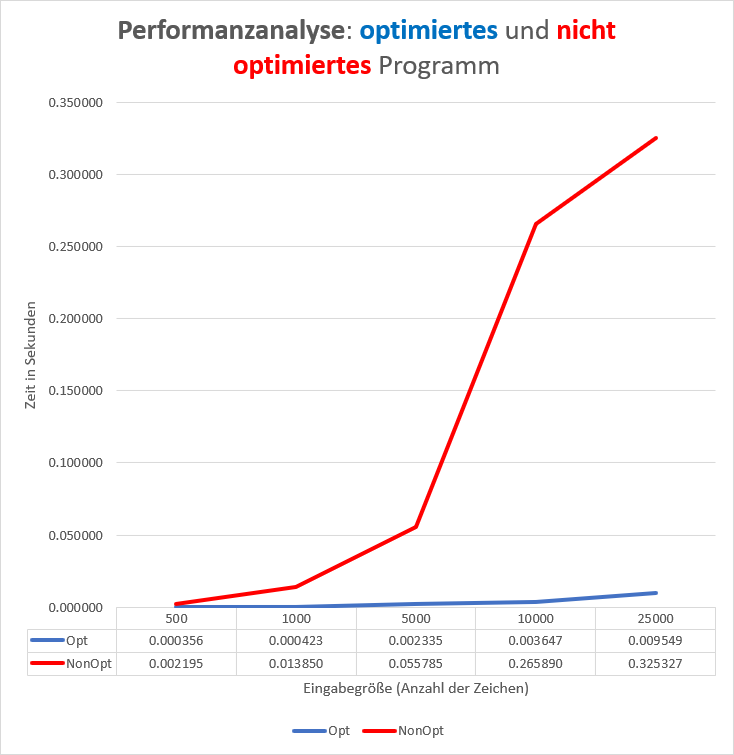
\includegraphics[width = \textwidth]{Figures/Performance.png}
    \caption{Performanzanalyse}
    \label{fig:perf}
\end{figure}

\section{Zusammenfassung und Ausblick} \label{ss:fazit}


Unser Ziel war es selbständig die MD2-Hashfunktion in C zu Implementieren. Hashfunktionen werden heutzutage in vielen Bereichen verwenden und stellen einen essentiellen Bestandteil dar \cite{attack}. Diese verwenden Padding, Checksums und S-Boxen, um aus Daten beliebiger Größe einen Hashwert fester Länger zu generieren. Obwohl der MD2-Algorithmus heute nicht mehr als sicher gilt und seine Verwendung abnimmt, war es dennoch eine interessante Erfahrung diesen selbst zu implementieren. Wir haben einen tiefen Einblick in den Aufbau und die Einzelteile der Hashfunktion erhalten können und konnten auch selbst testen wie stark Optimierungen sich auf die Laufzeit auswirken. Hätten wir mehr Zeit gehabt würden wir vermehrt \texttt{SIMD}-Operationen verwenden - nicht nur für die \texttt{XOR}-Operationen. Dies hätte den Vorteil, dass mehr Vorgehen parallel ausgeführt werden können und beim Padding wir auch 16-Byte gerichtete Eingaben verwenden könnten. Hätte aber den Nachteil gehabt, dass wir in der Hashfunktion einen noch höheren Speicheroverhead hätten.

\bibliographystyle{plain}
\bibliography{Ausarbeitung}{}

\end{document}
